
\documentclass[a4paper]{article}
\usepackage[text={165mm,245mm}]{geometry}
\usepackage{graphicx}
\usepackage{subfigure}
\usepackage{ctex}
\usepackage{float} 
\usepackage{amsmath}
\usepackage{listings}
\usepackage{xcolor}
\definecolor{mygreen}{rgb}{0,0.6,0}  
\definecolor{mygray}{rgb}{0.5,0.5,0.5}  
\definecolor{mymauve}{rgb}{0.58,0,0.82}  
  
% RISC-V Assembler syntax and style for latex lstlisting package
% 
% These are risc-v commands as per our university (University Augsburg, Germany) guidelines.
%
% Author: Anton Lydike
%
% This code is in the public domain and free of licensing
\lstdefinelanguage[RISC-V]{Assembler}
{
  alsoletter={.}, % allow dots in keywords
  alsodigit={0x}, % hex numbers are numbers too!
  morekeywords=[1]{ % instructions
    lb, lh, lw, lbu, lhu,
    sb, sh, sw,
    sll, slli, srl, srli, sra, srai,
    add, addi, sub, lui, auipc,
    xor, xori, or, ori, and, andi,
    slt, slti, sltu, sltiu,
    beq, bne, blt, bge, bltu, bgeu,
    j, jr, jal, jalr, ret,
    scall, break, nop
  },
  morekeywords=[2]{ % sections of our code and other directives
    .align, .ascii, .asciiz, .byte, .data, .double, .extern,
    .float, .globl, .half, .kdata, .ktext, .set, .space, .text, .word
  },
  morekeywords=[3]{ % registers
    zero, ra, sp, gp, tp, s0, fp,
    t0, t1, t2, t3, t4, t5, t6,
    s1, s2, s3, s4, s5, s6, s7, s8, s9, s10, s11,
    a0, a1, a2, a3, a4, a5, a6, a7,
    ft0, ft1, ft2, ft3, ft4, ft5, ft6, ft7,
    fs0, fs1, fs2, fs3, fs4, fs5, fs6, fs7, fs8, fs9, fs10, fs11,
    fa0, fa1, fa2, fa3, fa4, fa5, fa6, fa7
  },
  morecomment=[l]{;},   % mark ; as line comment start
  morecomment=[l]{\#},  % as well as # (even though it is unconventional)
  morestring=[b]",      % mark " as string start/end
  morestring=[b]'       % also mark ' as string start/end
}
% language definition

\lstset{ %  
  backgroundcolor=\color{white},   % choose the background color; you must add \usepackage{color} or \usepackage{xcolor}  
  basicstyle=\footnotesize,        % the size of the fonts that are used for the code  
  breakatwhitespace=false,         % sets if automatic breaks should only happen at whitespace  
  breaklines=true,                 % sets automatic line breaking  
  captionpos=bl,                    % sets the caption-position to bottom  
  commentstyle=\color{mygreen},    % comment style  
  deletekeywords={...},            % if you want to delete keywords from the given language  
  escapeinside={\%*}{*)},          % if you want to add LaTeX within your code  
  extendedchars=true,              % lets you use non-ASCII characters; for 8-bits encodings only, does not work with UTF-8  
  frame=single,                    % adds a frame around the code  
  keepspaces=true,                 % keeps spaces in text, useful for keeping indentation of code (possibly needs columns=flexible)  
  keywordstyle=\color{blue},       % keyword style  
  %language=Bin,                 % the language of the code  
  morekeywords={*,...},            % if you want to add more keywords to the set  
  numbers=left,                    % where to put the line-numbers; possible values are (none, left, right)  
  numbersep=5pt,                   % how far the line-numbers are from the code  
  numberstyle=\tiny\color{mygray}, % the style that is used for the line-numbers  
  rulecolor=\color{black},         % if not set, the frame-color may be changed on line-breaks within not-black text (e.g. comments (green here))  
  showspaces=false,                % show spaces everywhere adding particular underscores; it overrides 'showstringspaces'  
  showstringspaces=false,          % underline spaces within strings only  
  showtabs=true,                  % show tabs within strings adding particular underscores  
  stepnumber=1,                    % the step between two line-numbers. If it's 1, each line will be numbered  
  stringstyle=\color{orange},     % string literal style  
  tabsize=2,                       % sets default tabsize to 2 spaces  
  %title=myPython.py                   % show the filename of files included with \lstinputlisting; also try caption instead of title  
}  
\title{\heiti 
CODH - 单周期CPU设计 \hspace{0.3cm}实验报告}
\author{院系: \kaishu\underline{}\hspace{1.5cm}姓名: \kaishu \underline{}\hspace{1.5cm}学号: \kaishu \underline{}\hspace{1.5cm}}
\begin{document}
\maketitle

\section{实验目的}
\begin{itemize}
    \item 理解单周期CPU的结构和工作原理
    \item 掌握单周期CPU的设计和调试方法
    \item 熟练掌握数据通路和控制器的设计和Verilog描述方法
\end{itemize}

\section{实验环境}
\begin{itemize}
  \item macOS 13.0
  \item Rars1\_5.jar (Riscv Assembler and Runtime Simulator)
  \item Vivado 2019.3
  \item Nexys 4 DDR 开发板
\end{itemize}
\section{实验内容}
\subsection{设计CPU的数据通路(具备简单的I/O功能)和控制器}
\begin{itemize}
    \item 指令存储器和数据存储器均采用IP例化的分布式存储器,容量均为1024x32位,使用LabH3实验生成的COE文件初始化
    \item 寄存器堆增加一个用于调试的读端口,指令存储器和数据存储器均增加一个用于调试和初始化的读/写端口
    \item Led指示灯:输出程序运行状态或结果,MMIO地址0x3f00
    \item 时钟计数器:除复位清零外,一直对CPU工作时钟递增计数,用于测试程序执行时间,MMIO地址0x3f20  
  \end{itemize}

  \subsection{将CPU和SDU整合后下载至FPGA,进行逐条指令功能测试与进行排序程序测试}
  \begin{itemize}
    \item Led指示灯显示测试结果,或者排序程序耗费时钟周期数
    \item 查看电路资源使用情况和电路性能
  \end{itemize}
之后将指令和数据存储器用LabH3中的文件初始化后,与串行调试单元模块(SDU\_DM)整合,下载至FPGA中测试即可。

\section{逻辑设计 / 核心代码}
\subsection{设计CPU的数据通路(具备简单的I/O功能)和控制器}
\begin{itemize}
    \item 寄存器堆,增加一个用于调试的读端口
    \item 指令存储器、数据存储器,增加一个用于调试和初始化的读/写端口
    \item ALU运算器,可以通过修改Lab1中的ALU得到
    \item 立即数拓展器,依据不同的指令类型将立即数拓展为32位
    \item npc选择器
    \item 寄存器输入端选择器
    \item 控制信号生成器
    \item 跳转信号控制器、ALU信号控制器
  \end{itemize}

这些部件的设计是依照课本以及课件上给出的单周期CPU数据通路进行设计的,同时为了兼容SDU和实现MMIO进行了些许更改。
\begin{figure}[H]
    \centering
    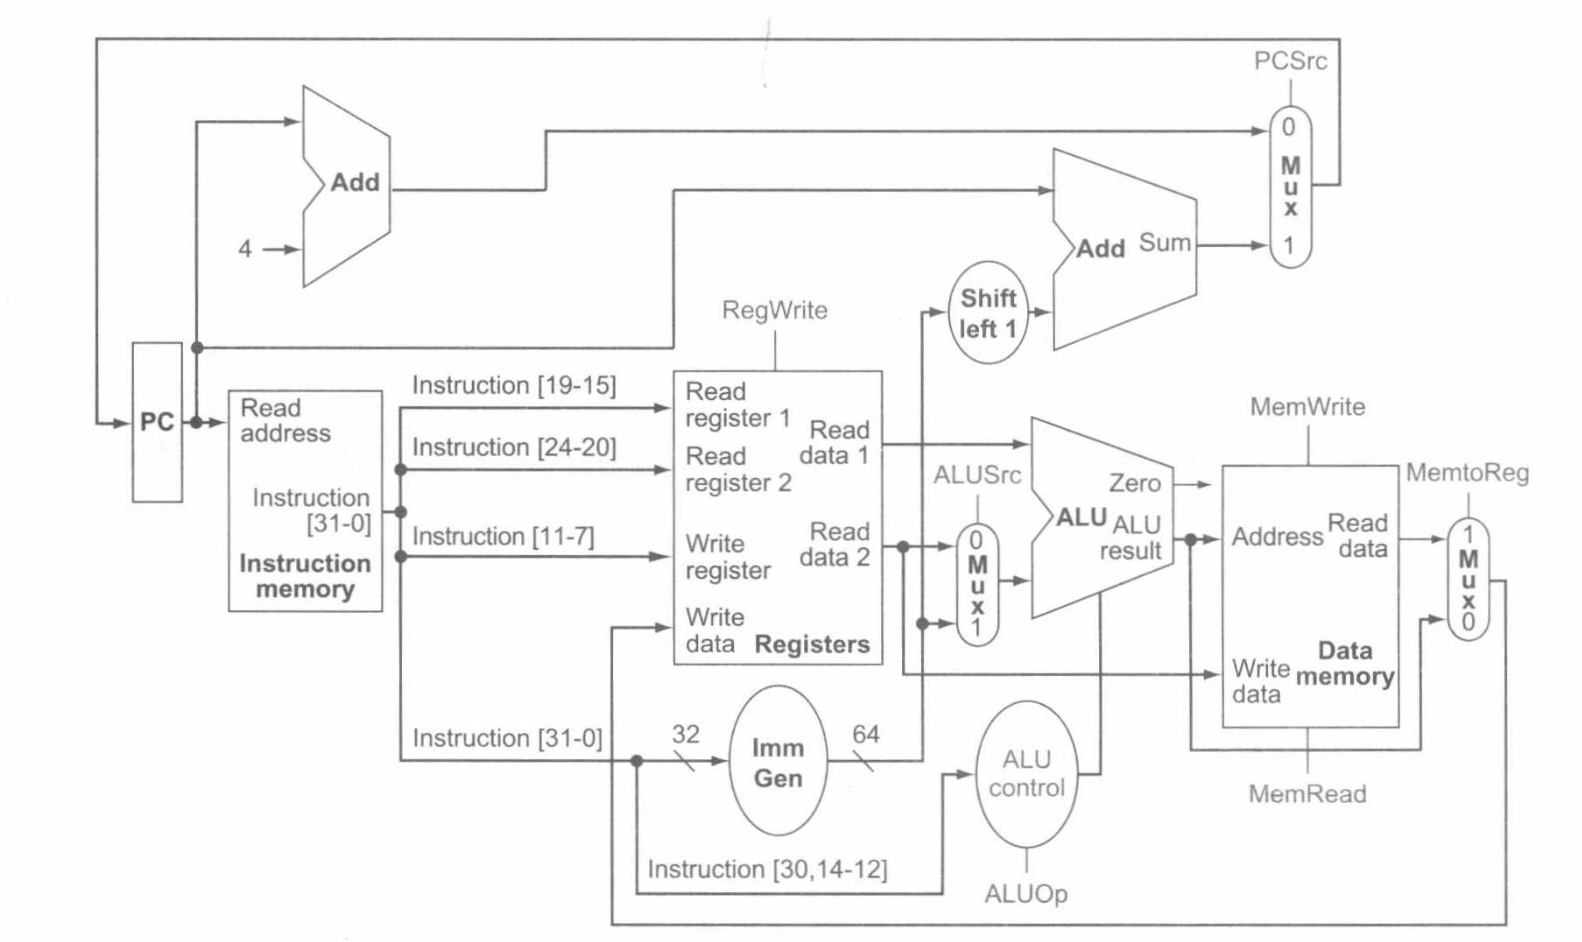
\includegraphics[width=0.9\textwidth]{1.png}
    \caption{CPU-fig}
    \label{fig:test1}
\end{figure}

需要注意的是,在npc选择器处对一些计算以及加法器进行了整合;在控制信号生成器中将ALU信号与跳转信号控制器单独做成了模块方便编写代码,
因此控制信号和实际的数据通路会也有所不同。

具体来说,这些模块的接口如下,模块内的具体实现请参见原始代码:

\begin{lstlisting}[language={verilog},title={cpu.v}] 
    module  reg_file(
        input  clk,		//时钟
        input [4:0]  ra0, ra1, ra2,	//读地址
        output [31:0] rd0, rd1, rd2,	//读数据
        input [4:0]  wa,		//写地址
        input [31:0] wd,	//写数据
        input we		//写使能
    );
    data_mem_inst(.a(), .d(), .clk(), .we(), .spo()); //这是ip核,对CPU和SDU都要实现读写,因此选择单端口,使用控制信号决定信号来自何处
    inst_mem_inst(.a(), .d(), .dpra(), .clk(), .we(), .spo(), .dpo()); //这是ip核,对CPU只需读,对SDU需要实现读写,因此选择双端口,分别接入CPU和SDU的信号
    module alu (
        input [31:0] a, b,     //两操作数
        input [2:0] f,            //功能选择
        output reg [31:0] y,     //运算结果
        output reg [2:0] t            //比较标志
    );
    module imm_gen (
        input [31:0] raw,
        input [6:0] opcode,
        input [2:0] funct3,
        output reg [31:0] ext_imm
    ); 
    module next_pc_sel(
        input [2:0] pc_sel,
        input [31:0] alu_out,
        input [31:0] pc,
        input [31:0] ext_imm,
        output reg [31:0] npc
    );
    module reg_file_sel(
        input [2:0] reg_sel,
        input [31:0] alu_out,
        input [31:0] pc,
        input [31:0] dm_rd,
        input [31:0] ext_imm,
        output reg [31:0] rf_wd
    );
    module control(
        input [6:0] opcode,
        input [2:0] cc,
        input [2:0] funct3,
        input [6:0] funct7,
        output branch,
        output reg [2:0] reg_sel,
        output reg [2:0] pc_sel,
        output reg mem_write,
        output reg alu_src,
        output [2:0] alu_op,
        output reg reg_write
    );
    module branch_control(
        input [6:0] opcode,
        input [2:0] cc,
        input [2:0] funct3,
        output reg branch
    );
    module alu_control(
        input [6:0] opcode,
        input [2:0] funct3,
        input [6:0] funct7,
        output reg [2:0] alu_op
    );
 \end{lstlisting}

有关MMIO的实现,主要在检测到数据存储器的地址输入信号为MMIO地址时,设置mmio\_flag,则此时数据存储器的写信号切换为零,同时在外部处理对mmio寄存器的读写。
具体代码如下:
\begin{lstlisting}[language={verilog},title={cpu.v}] 
    always@(*) begin        
        if ((dm_addr == 16'h7f00) || (dm_addr == 16'h7f20)) begin
            mmio_flag = 1;
        end
        else begin
            mmio_flag = 0;
        end
    end
    ...
    assign dm_we = ~flag ? (mmio_flag ? 0 : mem_write) : _we_dm;
    ...
    if(mem_write) begin
        if (dm_addr == 16'h7f00) begin
            led <= dm_d;
        end
        if (dm_addr == 16'h7f20) begin
            clock <= dm_d;
        end
    end
\end{lstlisting}
对于NPC选择器以及寄存器输入端选择器,总共有如下五种选择,只需要依照对应的参数切换即可。
\begin{lstlisting}[language={verilog},title={control.v}] 
    parameter ALU_OUT = 3'b000;
    parameter MEM_OUT = 3'b001; 
    parameter NEXT_PC = 3'b010; //PC + 4
    parameter IMM_PC = 3'b011;  //PC + IMM
    parameter IMM_ONLY = 3'b100; //IMM
 \end{lstlisting}

另外由于需要实现SDU对数据存储器与指令存储器的读写,这个cpu中会根据SDU输入的debug信号来切换读写信号的来源,如下:
\begin{lstlisting}[language={verilog},title={reg.v}] 
    wire flag;
    assign flag = debug;
    assign dm_addr = ~flag ? alu_out[11:2] : _w_addr;
    assign dm_d = ~flag ? rf_rd2 : _din;
    assign dm_we = ~flag ? (mmio_flag ? 0 : mem_write) : _we_dm;
    assign dm_clk = ~flag ? clk : _clk_ld;
    data_mem data_mem_inst(.a(dm_addr), .d(dm_d), .clk(dm_clk), .we(dm_we), .spo(dm_rd));
 \end{lstlisting}

最后,SDU调试时还要输出各类控制信号以及数据通路信息,需要将这些信号一一接给输出端,较为繁琐且没有难点,在这里不展示核心代码。

\subsection{将CPU和SDU整合后下载至FPGA,进行逐条指令功能测试与进行排序程序测试}
这里需要小幅修改LabH3中得到的测试程序。例如添加对MMIO的读写,用led来显示测试成功/失败。

烧录后测试程序以及排序程序的正确性已经由助教检查完成,单周期CPU设计任务完成。

\subsubsection{结果分析}
RTL电路:
\begin{figure}[H]
    \centering
    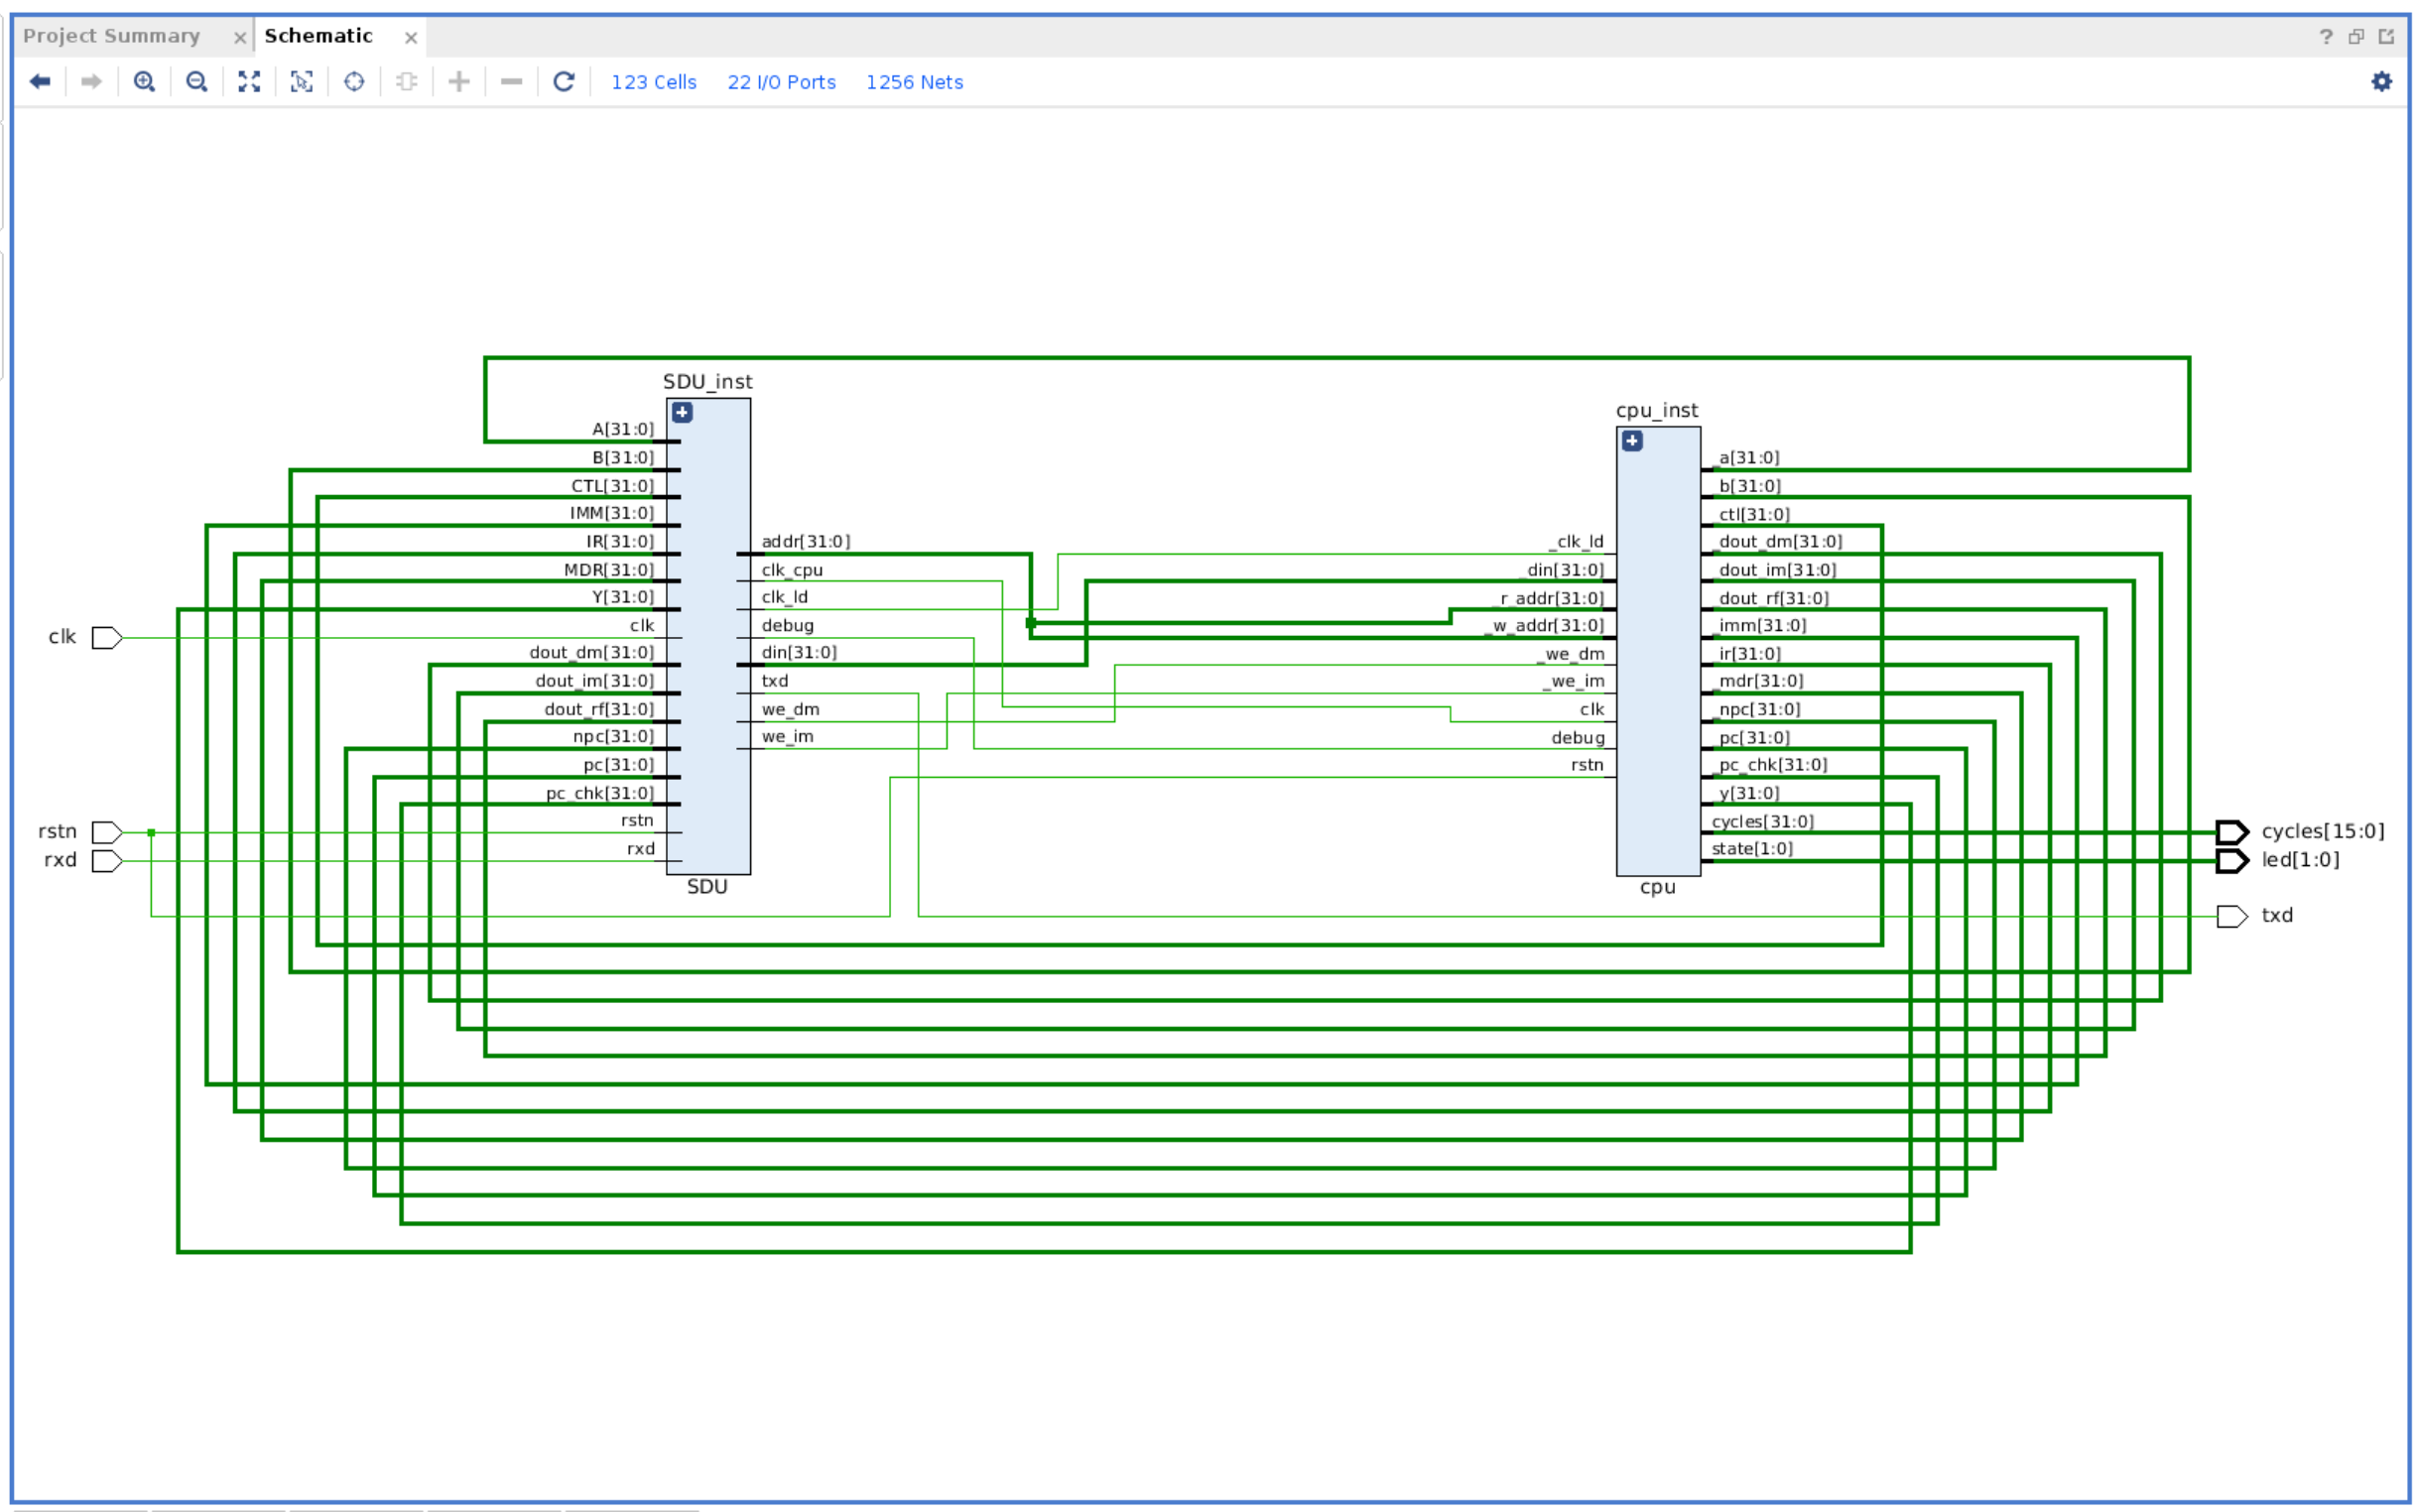
\includegraphics[width=0.9\textwidth]{2.png}
    \caption{RTL}
    \label{fig:test1}
\end{figure}

电路资源使用情况:
\begin{figure}[H]
    \centering
    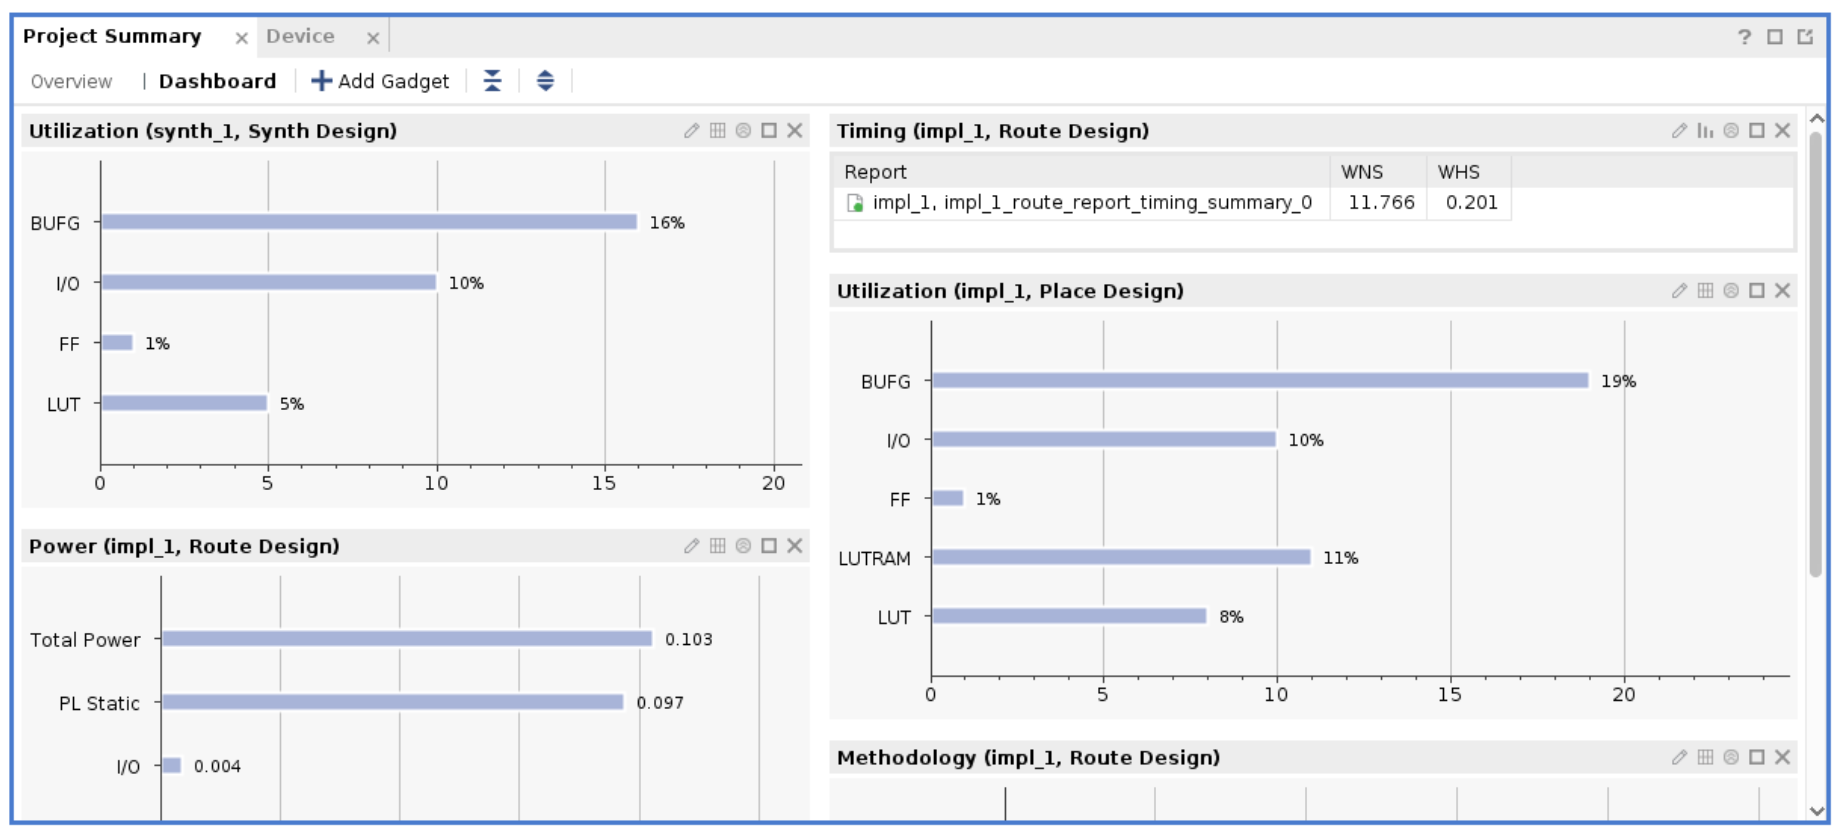
\includegraphics[width=0.9\textwidth]{3.png}
    \caption{UTL1}
    \label{fig:test1}
\end{figure}
\begin{figure}[H]
    \centering
    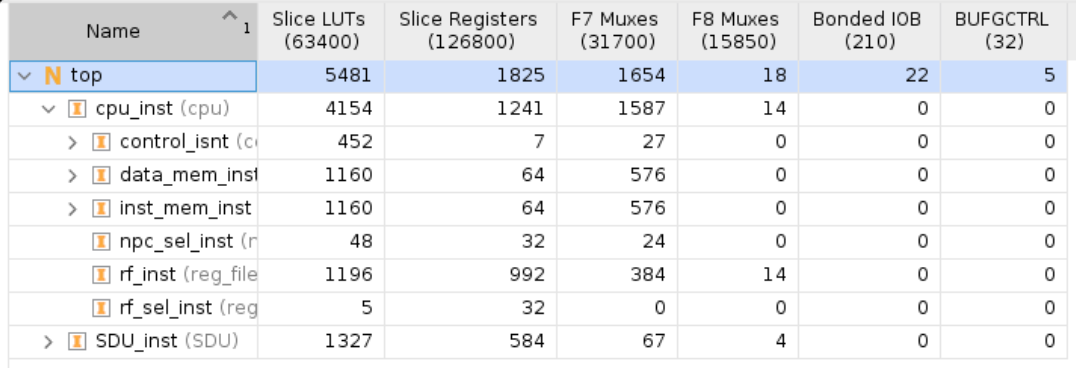
\includegraphics[width=0.9\textwidth]{4.png}
    \caption{UTL2}
    \label{fig:test1}
\end{figure}

电路性能:
\begin{figure}[H]
    \centering
    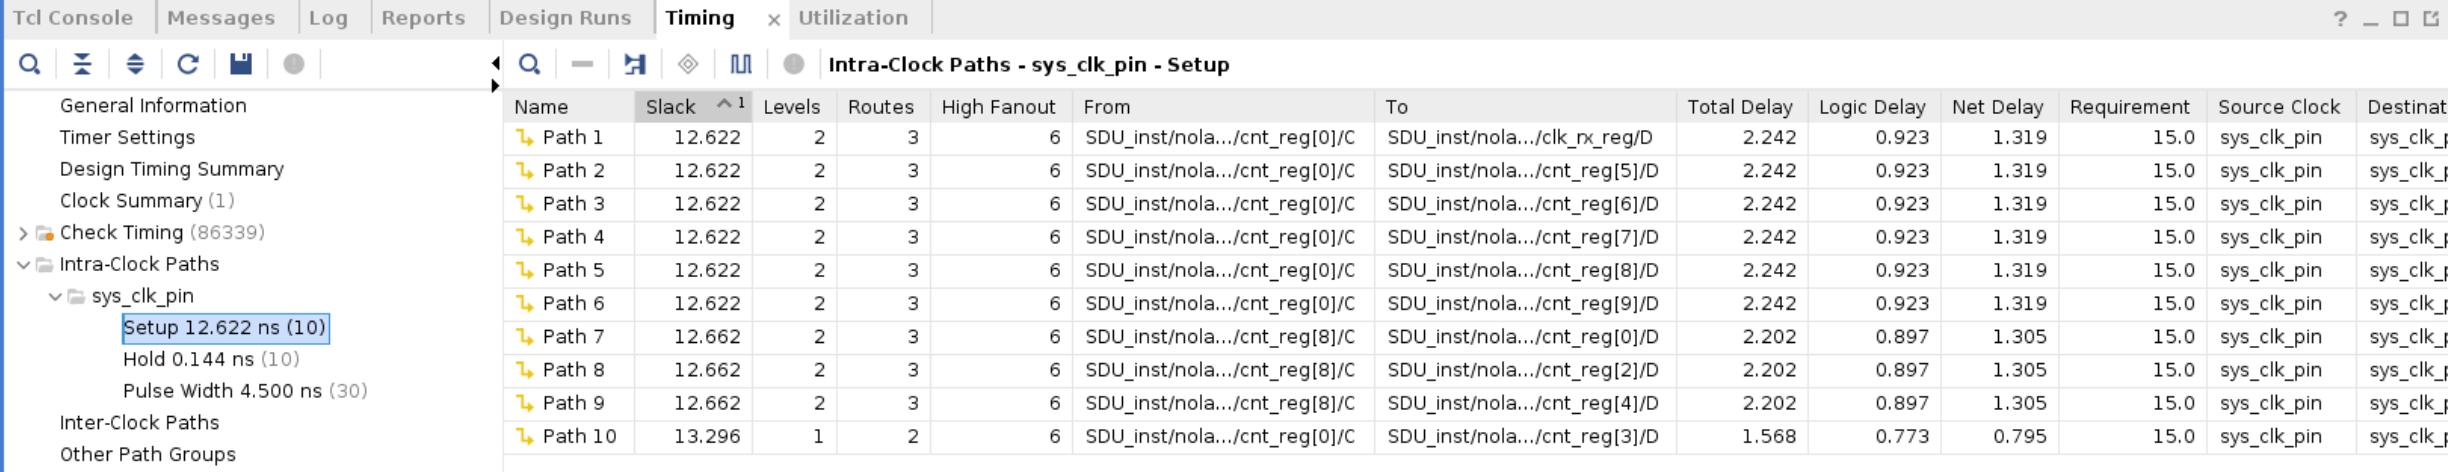
\includegraphics[width=0.9\textwidth]{5.png}
    \caption{TIMING}
    \label{fig:test1}
\end{figure}

\section {实验总结}
\begin{enumerate}
  \item 通过本次实验,我学习到了如何依据需求设计CPU的数据通路,如何划分模块以及设计控制信号以完成需求。
  \item 同时也学习了有关MMIO的知识,通过MMIO可以轻松地控制外设辅助显示必要信息。
  \item 本次实验思维难度不大,主要难点在于模块过多过于复杂,需要提前想好如何接各个模块之间的信号以及整体设计,否则编写代码会十分困难。
\end{enumerate}
\section {意见/建议}
无,这个实验设计很完美。
\end{document}